\section{Rank 1 theories}\label{sec:rank1theories}

In this section, we will compute the BPS partition functions of rank-1 5d theories by bootstrapping with the blowup equations. All rank-1 theories can be obtained via RG flows, which integrate out massive hypermultiplets, from three KK theories that come from 6d SCFTs compactified on a circle with/without twists. When a theory admits solvable blowup equations with consistent magnetic fluxes, all the IR theories descending from this UV theory by RG flows are guaranteed to have solvable blowup equations. So we will show that the blowup equations for all the rank-1 KK theories can be solved and the solutions are consistent with the BPS spectra computed by other methods. This will prove that the BPS spectra of all rank-1 5d theories can be computed by solving the blowup equations. We will also compute the BPS partition function of a new rank-1 theory, which we call the local $\mathbb{P}^2+1\mathbf{Adj}$ theory, obtained from the $\mathcal{N}=2$ $SU(2)$ gauge theory at $\theta=\pi$ by integrating out an instantonic hypermultiplet.


\subsection{KK theories}
There are three rank-1 KK theories: the $SU(2)$ gauge theory with 8 fundamental hypermultiplets, the $\mathcal{N}=2$ $SU(2)$ gauge theory at $\theta=0,\pi$. We discuss them one by one. 

\subsubsection{\texorpdfstring{$SU(2)+8\mathbf{F}$}{SU(2) + 8F}}

The $SU(2)$ gauge theory with 8 fundamental hypermultiplets is a KK theory arising from the 6d rank-1 E-string theory compactified on a circle \cite{Witten:1995gx,Ganor:1996mu,Seiberg:1996bd}.
\begin{align}
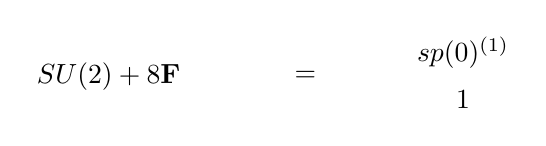
\begin{tikzpicture}
\draw (0, 0) node {$ SU(2) + 8\mathbf{F} $}
(2.5, 0) node {$ = $}
(4.5, 0.3) node {$ \mathfrak{sp}(0)^{(1)} $}
(4.5, -0.3) node {$ 1 $};
\end{tikzpicture}
\end{align}
The BPS partition function for this theory was computed in \cite{Hwang:2014uwa,Kim:2014dza} using the ADHM instanton string construction and also in \cite{Kim:2015jba,Kim:2017jqn} based in its 5-brane webs using topological vertex. It was also shown in \cite{Gu:2019pqj} that the elliptic genus of the 6d E-string theory is consistent with the blowup equation. 

We shall here solve the blowup equation in perspective of the 5d gauge theory. The prepotential on the Coulomb branch is given by
\begin{align}
6\mathcal{F} =6m_0 \phi^2+ 8\phi^3 - \frac{1}{2} \sum_{i=1}^8 \Big((\phi + m_i)^3 + (\phi - m_i)^3\Big)\ ,
\end{align}
where $ m_0 $ is the gauge coupling and $ m_{i=1, \cdots, 8} $ are the mass parameters of fundamental hypermultiplets. Collecting the gauge/gravitational and the gauge/$SU(2)_R$ Chern-Simons terms, the effective prepotential on the $\Omega$-background is expressed as 
\begin{align}
\mathcal{E} &= \frac{1}{\epsilon_1 \epsilon_2} \qty(\mathcal{F} - \frac{\epsilon_1^2 + \epsilon_2^2}{48} \bigg(4\phi - \sum_{i=1}^8 \Big((\phi + m_i) + (\phi - m_i)\Big)\bigg) + \epsilon_+^2 \phi ) \nonumber \\
&= \frac{1}{\epsilon_1 \epsilon_2} \qty(\mathcal{F} +\frac{\epsilon_1^2+\epsilon_2^2}{4}\phi + \epsilon_+^2 \phi) \, .
\end{align}
The perturbative part of the GV-invariant is
\begin{align}
\mathcal{Z}_{\rm pert}(\phi,m_i;\epsilon_{1,2}) = {\rm PE}\left[-\frac{1+p_1p_2}{(1-p_1)(1-p_2)}e^{-2\phi}  + \frac{\sqrt{p_1p_2}}{(1-p_1)(1-p_2)}\sum_{i=1}^8e^{-(\phi\pm m_i)}\right] \, .
\end{align}

For this theory, we find a set of the consistent magnetic fluxes
\begin{align}
n \in \mathbb{Z} \, , \quad B_{m_0}=0 \, , \quad B_{m_i}=1/2 \ \ {\rm for} \ 1\leq i\leq 8 \, ,
\end{align}
which leads to a unity blowup equation. The unity blowup equation with the magnetic fluxes can be solved and the solution is summarized in Table~\ref{table:SU2_8F}. This result matches the elliptic genus of the rank-1 E-string theory computed in \cite{Kim:2014dza}.

\begin{table}
\centering
\begin{tabular}{|c|C{30ex}||c|C{30ex}|} \hline
	$ \mathbf{d} $ & $ \oplus N_{j_l, j_r}^{\mathbf{d}} (j_l, j_r) $ & $ \mathbf{d} $ & $ \oplus N_{j_l, j_r}^{\mathbf{d}} (j_l, j_r) $  \\ \hline
	$ (1, 1) $ & $ 128(0, 0) $ & $ (1, 2) $ & $ 128(0, \frac{1}{2}) $ \\ \hline
	$ (1, 3) $ & $ 128(0, 1) $ & $ (2, 1) $ & $ 576(0, 0) \oplus 16(\frac{1}{2}, \frac{1}{2}) $ \\ \hline
	$ (2, 2) $ & $ 1942(0, \frac{1}{2}) \oplus (\frac{1}{2}, 0) \oplus 121(\frac{1}{2}, 1) \oplus (1, \frac{3}{2}) $ & $ (2, 3) $ & $ 560(0, 0) \oplus 4960(0, 1) \oplus 16(\frac{1}{2}, \frac{1}{2}) \oplus 576(\frac{1}{2}, \frac{3}{2}) \oplus 16(1, 2) $ \\ \hline
\end{tabular}
\caption{BPS spectrum of $ SU(2) + 8\mathbf{F} $ theory for $ d_1 \leq 2 $ and $ d_2 \leq 3 $. Here, $ \mathbf{d} = (d_1, d_2) $ labels BPS states with charge $ d_1 m_0 + d_2 \phi $. For convenience, we set all flavor mass parameters $ m_{i=1, \cdots, 8} $ to zero.} \label{table:SU2_8F}
\end{table}


\subsubsection{\texorpdfstring{$SU(2)_0+1\mathbf{Adj}$}{SU(2)0 + 1Adj}}

The compactification of the 6d rank-1 M-string theory on a circle gives rise to the 5d $SU(2)$ gauge theory at $\theta=0$ with an adjoint hypermultiplet preserving $\mathcal{N}=2$ supersymmetry,
\begin{align}
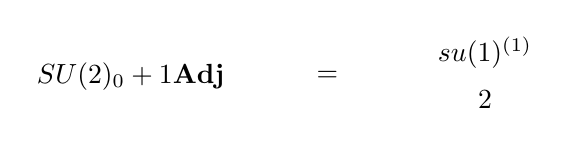
\begin{tikzpicture}
\draw (0, 0) node {$ SU(2)_0 + 1\mathbf{Adj} $}
(2.5, 0) node {$ = $}
(4.5, 0.3) node {$ \mathfrak{su}(1)^{(1)} $}
(4.5, -0.3) node {$ 2 $};
\end{tikzpicture}
\end{align}
The validity of the blowup equation for this theory was previously checked in \cite{Gu:2019pqj}.

The cubic prepotential on the Coulomb branch where $2\phi\pm m_1\ge0$ with $\phi>0$ is
\begin{align}
6\mathcal{F} = 6m_0 \phi^2+ 8\phi^3 - \frac{1}{2} \qty((2\phi + m_1)^3 + (2\phi - m_1)^3)  \ ,
\end{align}
where $m_0$ is the gauge coupling and $ m_1 $ is the mass parameter of the adjoint hypermultiplet.
The effective prepotential on $\Omega$-background is then given by
\begin{align}\label{eq:eff-pre-su2-adj}
\mathcal{E} &= \frac{1}{\epsilon_1 \epsilon_2} \qty(\mathcal{F} - \frac{\epsilon_1^2 + \epsilon_2^2}{48} \Big(4\phi - \big((2\phi + m_1) + (2\phi - m_1)\big)\Big) + \epsilon_+^2 \phi ) \nonumber \\
&=\frac{1}{\epsilon_1 \epsilon_2} \qty(\mathcal{F} +\epsilon_+^2\phi) \, .
\end{align}
The perturbative part of the GV-invariant is
\begin{align}\label{eq:pert-su2-adj}
	\mathcal{Z}_{\rm pert}(\phi,m_1;\epsilon_{1,2}) = {\rm PE}\left[-\frac{1+p_1p_2}{(1-p_1)(1-p_2)}e^{-2\phi}  + \frac{\sqrt{p_1p_2}}{(1-p_1)(1-p_2)}e^{-(2\phi\pm m_1)}\right] \, .
\end{align}

One can formulate a unity blowup equation for this theory using the following consistent magnetic fluxes. 
\begin{align}\label{eq:flux-su2-adj}
	n\in\mathbb{Z} \, , \quad B_{m_0}=0 \, , \quad B_{m_1}=1/2 \, .
\end{align}
The solution to the blowup equation is presented in Table~\ref{table:SU2_0_1Adj}. The result indeed matches the $\mathcal{N}=2$ $SU(2)_0$  instanton partition function computed using the ADHM calculus in \cite{Hwang:2014uwa}.
\begin{table}
	\centering
	\begin{tabular}{|c|C{27ex}||c|C{27ex}|} \hline
		$ \mathbf{d} $ & $ \oplus N_{j_l, j_r}^{\mathbf{d}} (j_l, j_r) $ & $ \mathbf{d} $ & $ \oplus N_{j_l, j_r}^{\mathbf{d}} (j_l, j_r) $  \\ \hline
		$ (1, 2, -2) $ & $ (0, \frac{1}{2}) $ & $ (1, 2, -1) $ & $ (0, 0) \oplus (0, 1) \oplus (\frac{1}{2}, \frac{1}{2}) $ \\ \hline
		$ (1, 2, 0) $ & $ 2(0, \frac{1}{2}) \oplus (\frac{1}{2}, 0) \oplus (\frac{1}{2}, 1) $ & $ (1, 4, -2) $ & $ (0, \frac{3}{2}) $ \\ \hline
		$ (1, 4, -1) $ & $ (0, 1) \oplus (0, 2) \oplus (\frac{1}{2}, \frac{3}{2}) $ & $ (1, 4, 0) $ & $ 2(0, \frac{3}{2}) \oplus  (\frac{1}{2}, 1) \oplus (\frac{1}{2}, 2)$ \\ \hline
		$ (2, 2, -3) $ & $ (0, 0) $ & $ (2, 2, -2) $ & $ 2(0, \frac{1}{2}) \oplus (\frac{1}{2}, 0) \oplus (\frac{1}{2}, 1) $ \\ \hline
		$ (2, 2, -1) $ & $ 4(0,0) \oplus 2(0,1) \oplus 3(\frac{1}{2},\frac{1}{2}) \oplus (\frac{1}{2},\frac{3}{2}) \oplus (1,1) $ & $ (2, 2, 0) $ & $ 5(0,\frac{1}{2}) \oplus (0,\frac{3}{2}) \oplus 3(\frac{1}{2},0)\oplus 3(\frac{1}{2},1) \oplus (1,\frac{1}{2}) \oplus (1,\frac{3}{2}) $ \\ \hline
		$ (2, 4, -3) $ & $ (0,1) \oplus (0,2) \oplus (\frac{1}{2},\frac{3}{2}) $ & $ (2, 4, -2) $ & $ 2(0,\frac{1}{2}) \oplus 4(0,\frac{3}{2}) \oplus (0,\frac{5}{2}) \oplus 3(\frac{1}{2},1) \oplus 	3(\frac{1}{2},2) \oplus (1,\frac{3}{2}) \oplus (1,\frac{5}{2}) $ \\ \hline
		$ (2, 4, -1) $ & $ (0,0) \oplus 7(0,1) \oplus 6(0,2) \oplus 3(\frac{1}{2},\frac{1}{2}) \oplus
		8(\frac{1}{2},\frac{3}{2}) \oplus 3 (\frac{1}{2},\frac{5}{2}) \oplus 2(1,1) \oplus 3(1,2) \oplus
		(1,3) \oplus (\frac{3}{2},\frac{5}{2}) $ & $ (2, 4, 0) $ & $ 5(0,\frac{1}{2}) \oplus 10(0,\frac{3}{2}) \oplus 3(0,\frac{5}{2}) \oplus (\frac{1}{2},0) \oplus 8(\frac{1}{2},1) \oplus 8(\frac{1}{2},2) \oplus (\frac{1}{2},3) \oplus (1,\frac{1}{2}) \oplus 4(1,\frac{3}{2}) \oplus 3(1,\frac{5}{2}) \oplus (\frac{3}{2},2)\oplus (\frac{3}{2},3) $ \\ \hline
	\end{tabular}
	\caption{BPS spectrum of $ SU(2)_0 + 1\mathbf{Adj} $ theory for $ d_1 \leq 2 $ and $ d_2 \leq 4 $. Here, $ \mathbf{d} = (d_1, d_2, d_3) $ labels the BPS states with charge $ d_1 m_0 + d_2 \phi + d_3 m_1 $. The states related by the symmetry $ d_3 \leftrightarrow -d_3 $ are omitted in the table.} \label{table:SU2_0_1Adj}
\end{table}


\subsubsection{\texorpdfstring{$SU(2)_\pi+1\mathbf{Adj}$}{SU(2)pi + 1Adj}}\label{sec:su2pi+1adj}

The 5d KK-theory $ SU(2)_\pi + 1\mathbf{Adj} $ is obtained by a circle compactification of the 6d $\mathcal{N}=(2,0)$ $A_2$ theory with $ \mathbb{Z}_2 $ outer automorphism twist \cite{Tachikawa:2011ch},
\begin{align}
\begin{tikzpicture}
\draw (0, 0) node {$ SU(2)_\pi + 1\mathbf{Adj} $}
(2.5, 0) node {$ = $}
(4.5, 0.3) node {$ \mathfrak{su}(1)^{(1)} $}
(4.5, -0.3) node {$ 2 $};
\draw (4.2, -0.5) .. controls (3.8, -1.2) and (5.2, -1.2) .. (4.8, -0.5);
\end{tikzpicture}
\end{align}
This theory has no conventional geometric description \cite{Bhardwaj:2019fzv}.

The perturbative spectrum cannot distinguish whether $\theta=0$ or $\theta=\pi$ for the $SU(2)$ gauge group. Thus the effective prepotential and the perturbative GV-invariant of this theory are the same as \eqref{eq:eff-pre-su2-adj} and \eqref{eq:pert-su2-adj}, respectively, for the $SU(2)_0+1{\bf Adj}$ theory. Naively, this means that the blowup equation of this theory is the same as that of the theory at $\theta=0$. However, it turns out that there are two independent blowup equations from the same effective prepotential but distinguished by two different sets of consistent magnetic fluxes. Instead of the fluxes given in \eqref{eq:flux-su2-adj} for the theory at $\theta=0$, this theory at $\theta=\pi$ has another set of consistent magnetic fluxes quantized as
\begin{equation}
	n \in \mathbb{Z} + 1/2 \, , \quad B_{m_0}=0 \, , \quad B_{m_1}=1/2 \, .
\end{equation}

These magnetic fluxes provide a unity blowup equation. Some leading BPS invariants we computed using the blowup equation are listed in Table~\ref{table:SU2_pi_1Adj}, which are indeed different from the BPS spectrum of the theory at $\theta=0$. This result also matches the instanton partition function using the ADHM quantum mechanics in \cite{Hwang:2014uwa}. This is our first example showing that  our bootstrap approach can be applied for the BPS spectrum computation for non-geometric theories.
\begin{table}[t]
	\centering
	\begin{tabular}{|c|C{26ex}||c|C{26ex}|} \hline
		$ \mathbf{d} $ & $ \oplus N_{j_l, j_r}^{\mathbf{d}} (j_l, j_r) $ & $ \mathbf{d} $ & $ \oplus N_{j_l, j_r}^{\mathbf{d}} (j_l, j_r) $  \\ \hline
		$ (1, 1, -2) $ & $ (0, 0) $ & $ (1, 1, -1) $ & $ (0, \frac{1}{2}) \oplus (\frac{1}{2}, 0) $ \\ \hline
		$ (1, 1, 0) $ & $ 2(0, 0) \oplus (\frac{1}{2}, \frac{1}{2}) $ & $ (1, 3, -2) $ & $ (0, 1) $ \\ \hline
		$ (1, 3, -1) $ & $ (0, \frac{1}{2}) \oplus (0, \frac{3}{2}) \oplus (\frac{1}{2}, 1) $ & $ (1, 3, 0) $ & $ 2(0, 1) \oplus (\frac{1}{2}, \frac{1}{2}) \oplus (\frac{1}{2}, \frac{3}{2}) $ \\ \hline
		$ (2, 2, -2) $ & $ (0,\frac{1}{2}) \oplus (\frac{1}{2},1) $ & $ (2, 2, -1) $ & $ (0,0) \oplus 2(0,1) \oplus 2(\frac{1}{2},\frac{1}{2})\oplus (\frac{1}{2},\frac{3}{2})\oplus (1,1) $ \\ \hline
		$ (2, 2, 0) $ & $ 3(0,\frac{1}{2}) \oplus (0,\frac{3}{2}) \oplus (\frac{1}{2},0) \oplus 3(\frac{1}{2},1) \oplus	(1,\frac{1}{2})\oplus (1,\frac{3}{2}) $ & $ (2, 4, -3) $ & $ (0,0) \oplus (0,2) \oplus (\frac{1}{2},\frac{3}{2}) $ \\ \hline
		$ (2, 4, -2) $ & $ 2(0,\frac{1}{2}) \oplus 3(0,\frac{3}{2}) \oplus (0,\frac{5}{2}) \oplus (\frac{1}{2},0) \oplus 2(\frac{1}{2},1) \oplus 3(\frac{1}{2},2) \oplus (1,\frac{3}{2})\oplus (1,\frac{5}{2}) $ & $ (2, 4, -1) $ & $ 4(0,0) \oplus 4(0,1) \oplus 6(0,2) \oplus 3(\frac{1}{2},\frac{1}{2}) \oplus 7(\frac{1}{2},\frac{3}{2}) \oplus 3(\frac{1}{2},\frac{5}{2}) \oplus 2(1,1) \oplus 3(1,2) \oplus (1,3) \oplus (\frac{3}{2},\frac{5}{2}) $ \\ \hline
		$ (2, 4, 0) $ & \multicolumn{3}{C{66ex}|}{$ 5(0,\frac{1}{2}) \oplus 8(0,\frac{3}{2}) \oplus 3(0,\frac{5}{2}) \oplus 3(\frac{1}{2},0) \oplus	6(\frac{1}{2},1) \oplus 8(\frac{1}{2},2) \oplus (\frac{1}{2},3) \oplus (1,\frac{1}{2}) \oplus 4(1,\frac{3}{2}) \oplus 3(1,\frac{5}{2}) \oplus (\frac{3}{2},2) \oplus (\frac{3}{2},3) $} \\ \hline
	\end{tabular}
	\caption{BPS spectrum of $ SU(2)_\pi + 1\mathbf{Adj} $ theory for $ d_1 \leq 2 $ and $ d_2 \leq 4 $. Here, $ \mathbf{d} = (d_1, d_2, d_3) $ labels BPS states with charge $ d_1 m_0 + d_2 \phi + d_3 m_1 $. The states related by the symmetry $ d_3 \leftrightarrow -d_3 $ are omitted in the table.} \label{table:SU2_pi_1Adj}
\end{table}


\subsection{5d SCFTs: Non-Lagrangian theories}
The BPS partition functions of all the rank-1 5d SCFTs which have no gauge theory descriptions, can be computed by solving the blowup equations. To show this we will consider two simple examples: a local $\mathbb{P}^2$ theory and a local $\mathbb{P}^2 +1{\bf Adj}$ theory.


\subsubsection{\texorpdfstring{Local $\mathbb{P}^2$}{LocalP2}}

This theory is a rank-1 SCFT with no mass parameter, which is engineered by compactification of M-theory on a local $\mathbb{P}^2$ embedded in a CY 3-fold. This theory is also called the $E_0$ theory. The blowup equation for the SCFT of a local $\mathbb{P}^2$ was solved in \cite{Huang:2017mis}. We shall briefly review this.

The effective prepotential of this theory on the $\Omega$-background is simply given by
\begin{align}
\mathcal{E} = \frac{1}{\epsilon_1 \epsilon_2} \qty(9\phi^3 - \frac{(\epsilon_1^2 + \epsilon_2^2)\phi}{8} + \epsilon_+^2 \phi) \, .
\end{align}
The CY 3-fold of a local $ \mathbb{P}^2 $ contains only one primitive curve class $\ell$ with  $\ell^2= +1 $. The volume of this curve is $ \vol (\ell) = 3\phi $. Thus the magnetic fluxes that couple to the curve should be quantized as 
\begin{align}\label{eq:P2_shift}
n\in \mathbb{Z} \pm 1/6 \quad {\rm or} \quad n\in \mathbb{Z} + 1/2 \, .
\end{align}
These are all the consistent magnetic fluxes. The blowup equation with $n\in \mathbb{Z} + 1/2$ is a vanishing blowup equations, whereas the other choices of fluxes lead to unity blowup equations \cite{Huang:2017mis}, and they are all solvable.
The solution to these blowup equations is summarized in Table~\ref{table:P2}.
\begin{table}[H]
	\centering
	\begin{tabular}{|c|C{30ex}||c|C{30ex}|} \hline
		$ d $ & $ \oplus N_{j_l, j_r}^d (j_l, j_r) $ & $ d $ & $ \oplus N_{j_l, j_r}^d (j_l, j_r) $ \\ \hline
		$ 1 $ & $ (0, 1) $ & $ 2 $ & $ (0, \frac{5}{2}) $ \\ \hline
		$ 3 $ & $ (0, 3) \oplus (\frac{1}{2}, \frac{9}{2}) $  & $ 4 $ & $ \! (0, \frac{5}{2}) \oplus (0, \frac{9}{2}) \oplus (0, \frac{13}{2}) \oplus (\frac{1}{2}, 4) \oplus (\frac{1}{2}, 5) \oplus (\frac{1}{2}, 6) \oplus (1, \frac{11}{2}) \oplus (\frac{3}{2}, 7) \! $ \\ \hline
	\end{tabular}
	\caption{BPS spectrum of a local $ \mathbb{P}^2 $ for $ d \leq 4 $. Here, $ d $ labels the BPS states wrapping the degree $d$ curve in $\mathbb{P}^2$.} \label{table:P2}
\end{table}


\subsubsection{\texorpdfstring{Local $\mathbb{P}^2 + 1\mathbf{Adj}$}{Local P2 + 1Adj}}
The local $\mathbb{P}^2$ + 1$\mathbf{Adj}$ (or $``SU(2)_\pi+1\mathbf{Adj}-1\mathbf{F}"$) theory was first proposed in \cite{Bhardwaj:2019jtr}. This theory can be obtained by an RG flow from the UV $SU(2)_\pi+1{\bf Adj}$ theory after integrating out an instantonic hypermultiplet.

One way to see the existence of this theory is as follows. Recall that the SCFT of a local $\mathbb{P}^2$ (or the $E_0$ theory) can be obtained by blowing down an exceptional curve in a Hirzebruch surface $\mathbb{F}_1$. This corresponds to integrating out an instantonic hypermultiplet in the pure $SU(2)_\pi$ theory. In this regard, the $E_0$ theory can be thought of as ``$SU(2)_\pi-1\mathbf{F}$'' since we are ``subtracting'' a hypermultiplet. Likewise, the $SU(2)_\pi + 1\mathbf{Adj}$ theory we discussed in section \ref{sec:su2pi+1adj} has a hypermultiplet with charge ${\bf d}=(1,1,-2)$ at the 1-instanton sector and integrating out this hypermultiplet induces an RG flow to a consistent rank-1 SCFT with one mass parameter. We will call this IR SCFT  the local $\mathbb{P}^2+1\mathbf{Adj}$ theory. This theory is a non-Lagrangian theory. Here $+1\mathbf{Adj}$ simply means this theory contains a hypermultiplet originating from the adjoint hypermultiplet in its parent $SU(2)_\pi+1{\bf Adj}$ theory. The adjoint hypermultiplet in this SCFT can also be integrated out to give the SCFT of a local $\mathbb{P}^2$.

This theory is also a non-geometric theory. However, there is a 5-brane web for this theory with an $O7^+$-plane where the hypermultiplet associated with an $O7^+$-plane is in the symmetric representation of $SU(2)$ that is equivalent to the adjoint of the UV $SU(2)$ gauge symmetry. A simple way to construct the corresponding 5-brane web is to attach an $O7^+$-plane to a 5-brane web for the pure $SU(2)_\pi$ theory, as depicted in Figure \ref{fig:SU2_pi_adj_F_web}. (See also Appendix \ref{sec:appendix2} for more details of obtaining a 5-brane web for the $SU(2)_\pi + 1\mathbf{Adj}$ theory.)

The hypermultiplet which we will integrate out is the $(p,q)$-string state associated with the edge of the length $-\phi-m_0+2m_1$ in the brane web. Integrating out this hypermultiplet corresponds to taking the infinite length limit of the edge $-\phi-m_0+2m_1\rightarrow\infty$ while the lengths of other edges are kept finite. After this, we will get a 5-brane web for the local $\mathbb{P}^2+``1\mathbf{Adj}"$ theory. In this 5-brane web diagram, one can also see that by taking another limit $m_1 - 2\phi\rightarrow \infty$, after taking the limit $-\phi-m_0+2m_1\rightarrow\infty$, the diagram reduces to the brane web for a local $\mathbb{P}^2$, which is consistent with the expected RG flow for this theory.

\begin{figure}
	\centering
	\begin{tikzpicture}
	\draw[thick] (0, 0) -- (2, 0) -- (0, 2) -- (0, 0)
	(0, 0) -- (-0.5, -0.5)
	(2, 0) -- (3, -0.5)
	(-3, 0) -- (-4, -0.5)
	(0, 2) -- (-0.5, 3) -- (-0.5, 3.5)
	(-0.5, 3) -- (-1, 3.5);
	\draw[dashed] (-5, -0.5) -- (4, -0.5);
	\filldraw[fill=white, thick] (-0.5, -0.5) circle (0.15);
	\draw (1, -0.2) node {\scriptsize{$ {3\phi + m_0 - 2m_1} $}}
	(0.9, 2.6) node {\scriptsize{$ {-\phi - m_0 + 2m_1} $}}
	(-0.9, -0.1) node {\scriptsize{$ {m_1 - 2\phi} $}}
	(-0.5, -0.9) node {\scriptsize{$O7^+$}}
	;
	\end{tikzpicture}
	\caption{A 5-brane web for $SU(2)_\pi+1\mathbf{Adj}$, where a flop transition associated with the $e$ curve in $\mathbb{P}^2$ is performed.} \label{fig:SU2_pi_adj_F_web}
\end{figure}
We will now compute the partition function using the chamber for the brane web of the $SU(2)_\pi+1{\bf Adj}$ theory depicted in Figure~\ref{fig:SU2_pi_adj_F_web}. It is convenient to reparameterize the parameters in the brane web as follows:
\begin{align}
\tilde{\phi} = \phi + \frac{1}{3}m_0 - \frac{2}{3} m_1 \, , \quad
\tilde{m} = \frac{2}{3} m_0 - \frac{1}{3} m_1 \, ,
\end{align}
so that the volumes of 2-cycles in Figure~\ref{fig:SU2_pi_adj_F_web} become
\begin{align}
&3\phi + m_0 - 2m_1 = 3\tilde{\phi} \, , \quad
m_1 - 2\phi = \tilde{m} - 2\tilde{\phi} \, , \nonumber \\
&-\phi - m_0 + 2m_1 = -\tilde{\phi} + 2m_0 - 4\tilde{m} \, .
\end{align}

In order to get the IR  local $\mathbb{P}^2+1\mathbf{Adj}$ theory, we take the limit $ m_0 \to \infty $ while $ \tilde{\phi} $ and $ \tilde{m} $ are kept finite. The cubic prepotential and the mixed gravitational Chern-Simons level of the IR  theory can be obtained from those of the parent theory as
\begin{align}
\mathcal{F}_{IR}=\mathcal{F}_{UV} + \frac{1}{6}(\phi+m_0-2m_1)^3 \, , \quad C^G_{IR} =C^G_{UV} -2(\phi+m_0-2m_1) \, ,
\end{align}
whereas the mixed gauge/$SU(2)_R$ level $C^R$ remains the same along the RG flow. Thus the effective prepotential of a local  $\mathbb{P}^2+1\mathbf{Adj}$ on the extended Coulomb branch where $\tilde\phi>0$ and $\tilde{m}-2\tilde{\phi}\geq 0$ becomes 
\begin{align}
\mathcal{E} &= \frac{1}{\epsilon_1 \epsilon_2} \qty(\frac{3}{2}\tilde{\phi}^3 - \frac{(\epsilon_1^2 + \epsilon_2^2)\tilde{\phi}}{8} + \epsilon_+^2 \tilde{\phi} ) \, ,
\end{align}
up to the terms independent of $\tilde\phi$. Interestingly, this prepotential is the same as that of a local $\mathbb{P}^2$. However, they are different theories because the  $\mathbb{P}^2+1\mathbf{Adj}$ theory contains an additional hypermultiplet coming from the adjoint hypermultiplet of the parent theory, while the $E_0$ theory has no hypermultiplet. The GV-invariant for this hypermultiplet is thus a key input for solving the blowup equation
\begin{equation}
\mathcal{Z}_{\rm hyper}(\tilde{\phi},\tilde{m};\epsilon_{1,2}) = \PE \qty[\frac{\sqrt{p_1p_2}}{(1-p_1)(1-p_2)}e^{-(\tilde{m}- 2\tilde\phi)}] \, .
\end{equation}

The feasible magnetic fluxes that one can turn on are
\begin{align}
n \in \mathbb{Z}+ 1/6 \, , \quad B_{\tilde{m}} = -1/6 \, .
\end{align}
The blowup equation with this flux choice is a unity blowup equation. We solve this equation and find the BPS spectrum of the local  $\mathbb{P}^2+1\mathbf{Adj}$ theory listed in Table~\ref{table:SU2_pi_Adj-F}. As expected, this result also agrees with the RG flow from the BPS spetrum in the $SU(2)_\pi+1{\bf Adj}$ theory given in Table \ref{table:SU2_pi_1Adj} in the limit $-\tilde{\phi}+2m_0-4\tilde{m}\rightarrow \infty$ while $\tilde\phi$ and $\tilde{m}$ are kept finite.

\begin{table}
	\centering
	\begin{tabular}{|c|C{27ex}||c|C{27ex}|} \hline
		$ \mathbf{d} $ & $ \oplus N_{j_l, j_r}^{\mathbf{d}} (j_l, j_r) $ & $ \mathbf{d} $ & $ \oplus N_{j_l, j_r}^{\mathbf{d}} (j_l, j_r) $  \\ \hline
		$ (1, -2) $ & $ (0, 0) $ & $ (1, 1) $ & $ (0, \frac{1}{2}) \oplus (\frac{1}{2}, 0) $ \\ \hline
		$ (1, 4) $ & $ (0, 0) \oplus (0, 2) \oplus (\frac{1}{2}, \frac{3}{2}) $ & $ (1, 7) $ & $ (0,\frac{3}{2}) \oplus (0,\frac{5}{2}) \oplus (0,\frac{7}{2}) \oplus (\frac{1}{2},2) \oplus (\frac{1}{2},3) \oplus (\frac{1}{2},4) \oplus (1,\frac{7}{2}) $ \\ \hline
		$ (2, 2) $ & $ (0, \frac{1}{2}) \oplus (\frac{1}{2}, 1) $ & $ (2, 5) $ & $ 2(0,1) \oplus (0,2) \oplus (0,3) \oplus (\frac{1}{2},\frac{1}{2}) \oplus (\frac{1}{2},\frac{3}{2}) \oplus	2(\frac{1}{2},\frac{5}{2}) \oplus (1,2) \oplus (1,3) $ \\ \hline
		$ (2, 8) $ & \multicolumn{3}{C{63ex}|}{$ 2(0,\frac{1}{2}) \oplus 2(0,\frac{3}{2}) \oplus 6(0,\frac{5}{2}) \oplus 3(0,\frac{7}{2}) \oplus 4(0,\frac{9}{2}) \oplus 2(\frac{1}{2},1) \oplus 4(\frac{1}{2},2) \oplus 6(\frac{1}{2},3) \oplus 6(\frac{1}{2},4) \oplus 2(\frac{1}{2},5) \oplus (1,\frac{3}{2}) \oplus 3(1,\frac{5}{2}) \oplus 5(1,\frac{7}{2}) \oplus 4(1,\frac{9}{2}) \oplus (1,\frac{11}{2}) \oplus (\frac{3}{2},3) \oplus 2(\frac{3}{2},4) \oplus 2(\frac{3}{2},5) \oplus (2,\frac{9}{2}) \oplus (2,\frac{11}{2}) $} \\ \hline
	\end{tabular}
	\caption{BPS spectrum of  $\mathbb{P}^2+1\mathbf{Adj}$ theory with $ d_1 \leq 2 $ and $ d_2 \leq 9 $. Here, $ \mathbf{d} = (d_1, d_2) $ labels the BPS states with charge $d_1 \tilde{m} + d_2 \tilde{\phi} $.} \label{table:SU2_pi_Adj-F}
\end{table}